\documentclass{article}
\usepackage{graphicx} % Required for inserting images
\usepackage{multicol}
\usepackage{indentfirst}
\usepackage{blindtext}
\usepackage{algorithm}
\usepackage{multirow}
\usepackage{algorithmic}
\usepackage{titlesec}
\pagenumbering{roman}
\usepackage[table]{xcolor} % Allows defining of row colors
\usepackage{array}
\usepackage{lipsum}


\input{General/Preamble} % Loads in the preamble 
% Give your report a title

\newcommand\assignmenttitle{
CARE
}
\newcommand\reportmaintitle{
   Counterfactual-based Algorithmic Recourse for Explainable Pose
Correction
}
\newcommand\reporttitle{
   CARE : Counterfactual-based Algorithmic Recourse for Explainable Pose
Correction
}

% Insert course code, name, quartile number and year (or any other subtitle)
\newcommand\reportsubtitle{
Multimedia Content Analysis (CS6880)
}

% Add your group number (for DBL) or any other text.
\newcommand\groupnumber{
\textbf{ Group List}
}

% Insert authors and student numbers here
\newcommand\reportauthors{
Yug Patel & CS23MTECH14019 \\
}

% Add the name of your tutor (for DBL) or any other text.
\newcommand\grouptutor{
 
}

% Date and location (default: current date and Eindhoven)
\newcommand\placeanddate{
Eindhoven, \today
}

% Define Tue-red (color of the TU/e logo). Can be changed to drastically change the look of the template
\definecolor{Tue-red}{RGB}{199, 25, 24}

% All of the following code can be removed to be left with (close to) default LaTeX behaviour. 

% Sets up hyperlinks in the document to be colored
\hypersetup{
    colorlinks=true,
    linkcolor=Tue-red,
    urlcolor=Tue-red,
    citecolor = Tue-red
    }
\urlstyle{same} % Defines settings for link and reference formatting


% Change bullet style for level 1, 2 and 3 respectively for itemize
\renewcommand{\labelitemi}{\scriptsize\textcolor{Tue-red}{$\blacksquare$}}% level 1
\renewcommand{\labelitemii}{\scriptsize\textcolor{Tue-red}{$\square$}}% level 2
\renewcommand{\labelitemiii}{\textcolor{Tue-red}{$\circ$}}% level 3

% \renewcommand{\labelitemi}{\small\textcolor{Tue-red}{\ding{70}}} % level 1
% \renewcommand{\labelitemii}{\small\textcolor{Tue-red}{\ding{71}}}% level 2
% \renewcommand{\labelitemiii}{\tiny\textcolor{Tue-red}{\ding{71}}}% level 3

% Change bullet style for level 1, 2 and 3 respectively for enumerate
\renewcommand{\labelenumi}{\textbf{\textcolor{Tue-red}{\arabic*.}}}% level 1
\renewcommand{\labelenumii}{\textbf{\textcolor{Tue-red}{[\alph*]}}}% level 2
\renewcommand{\labelenumiii}{\textbf{\textcolor{Tue-red}{\roman*.}}}% level 3

% Have reference labels be linked to section (section 3 will have fig. 3.1 etc.)
\counterwithin{equation}{section} % For equations
\counterwithin{figure}{section} % For figures
\counterwithin{table}{section} % For tables

% Creates a beautiful header/footer
\pagestyle{fancy}
\lhead{\includegraphics[height = 16pt]{Images/IIT_Hyderabad.jpg}}
\rhead{\reporttitle}
\renewcommand{\footrulewidth}{0.4pt}
\cfoot{Page \thepage}

% Formats section, subsection and subsubsection titles respectively 
\titleformat{\section}{\sffamily\color{Tue-red}\Large\bfseries}{\thesection\enskip\color{gray}\textbar\enskip}{0cm}{} % Formats section titles

\titleformat{\subsection}{\sffamily\color{Tue-red}\large\bfseries}{\thesubsection\enskip\color{gray}\textbar\enskip}{0cm}{} % Formats subsection titles

\titleformat{\subsubsection}{\sffamily\color{Tue-red}\bfseries}{\thesubsubsection\enskip\color{gray}\textbar\enskip}{0cm}{} % Formats subsubsection titles

% Formats captions
\DeclareCaptionFont{Tue-red}{\color{Tue-red}}
\captionsetup{labelfont={Tue-red,bf}}

 % Changes font to mlmodern
\usepackage{mlmodern}

% Removes indent when starting a new paragraph
\setlength\parindent{0pt}

% Limits the ToC to sections and subsections (no subsubsec.)
\setcounter{tocdepth}{3}
 % Loads in user defined settings
\begin{document}

% Inserts the front page
\begin{titlepage}
\centering

\begin{tikzpicture}
\node[inner sep=0pt] (logo) at (0,0)
    {\includegraphics[width=.25\textwidth]{Images/IIT_Hyderabad.jpg}};
\end{tikzpicture}

\vspace{1cm}



\begin{tikzpicture}
\node[inner sep=0pt] (reportsubtitle1) at (0,0) {\sffamily\huge\textbf{ Indian Institute of Technology Hyderabad }};
\gettikzxy{(reportsubtitle1.west)}{\subtitlex}{\subtitley}
\gettikzxy{(reportsubtitle1.east)}{\titlex}{\titley}
\end{tikzpicture}

\vspace{2cm}




\begin{tikzpicture}
\node[inner sep=0pt,Tue-red] (reportsubtitle1) at (0,0) {\sffamily\huge\reportsubtitle};
\gettikzxy{(reportsubtitle1.west)}{\subtitlex}{\subtitley}
\gettikzxy{(reportsubtitle1.east)}{\titlex}{\titley}
\end{tikzpicture}

\vspace{2cm}

\begin{tikzpicture}
\node[inner sep=0pt] (logo) at (0,0){\sffamily\huge\assignmenttitle};
\node[text width = 0.7\textwidth, right = of logo](title){\sffamily\huge\reportmaintitle};
\gettikzxy{(title.south)}{\sffamily\subtitlex}{\subtitley}
\gettikzxy{(title.north)}{\titlex}{\titley}
\draw[line width=1mm, Tue-red]($(logo.east)!0.5!(title.west)$) + (0,\subtitley) -- +(0,\titley);
\end{tikzpicture}
% Authors
\vspace{1cm}
\sffamily\Large\textbf{Authors:}
\sffamily Bhat Dittakavi\textsuperscript{1}, Vineeth N Balasubramanian\textsuperscript{2}, et al.



% Paper Venture
\vspace{0.5cm}
\sffamily \Large \textbf{Paper Venue:}
\sffamily \large WACV 2024 \\

\vspace{1cm}

% \sffamily\groupnumber

\begin{table}[H]
\centering
\sffamily
\large
\begin{tabu} to 0.8\linewidth {cc}

\textbf{Name} & \textbf{Roll Number}\\

\hline

\sffamily\reportauthors

\end{tabu}

\end{table}

\sffamily \grouptutor
\vfill
\sffamily \Large \textcolor{white}{\placeanddate} \\


% Guided By
\vspace{0.5cm}
\sffamily \Large \textbf{Guided By:} \\
\sffamily \large Prof. C Krishna Mohan (IIT-Hyderabad) \\
\vspace{0.5cm}
\sffamily \Large \textbf{Teaching Assistant:} \\
\sffamily \large Manan Darji (M.Tech IIT-Hyderabad)

\end{titlepage}









\newpage

% Generates a ToC without page number
{\hypersetup{linkcolor=black} % Keeps the ToC black even with non-black linkcolor
\tableofcontents\thispagestyle{empty}}
\newpage

% % contains inspiration for formatting tables, images, text citations etc.
\section{ Motivation for the work.} \pagenumbering{roman}
\setlength{\parindent}{20pt}
\begin{itemize}
\item The realm of human pose correction stands as an underexplored frontier within the vast landscape of kinesiology-based applications. The surge in popularity of home-based fitness routines post-pandemic has sparked a heightened interest in innovative fitness monitoring solutions. This heightened interest stems from the realization that effective human pose monitoring not only enhances workout efficiency but also contributes significantly to preventing injuries and optimizing performance.

\item The growing demand for personalized fitness experiences has propelled human pose monitoring into the spotlight, making it a focal point in the domain of computer vision. Traditionally, efforts in this domain were predominantly centered around human pose classification for various applications. However, the evolution of technology and the shift towards holistic fitness management have underscored the need for precise and real-time human pose correction mechanisms.

\item The commercial importance of human pose correction cannot be overstated, especially in the context of wearable devices, virtual fitness trainers, and augmented reality applications. The ability to accurately assess and correct human posture not only enhances the user experience but also opens doors to new avenues in sports analytics, rehabilitation, and ergonomic design.

\item In light of these developments, exploring the intricacies of human pose correction not only addresses a critical research gap but also holds immense potential for practical applications across diverse sectors. It is within this context of burgeoning opportunities and technological advancements that the motivation to delve deeper into human pose correction arises, aiming to unravel its full potential in enhancing human performance and well-being.
\end{itemize}

\section{Problem Statement.}

\begin{multicols}{2}

	\begin{itemize}
    \item In the process of analyzing an image of an individual executing a pose, we utilize a pre-established pose estimator to create pose keypoints. Following that, we extract vectors representing the angles of the pose and categorize the pose into one of the ‘C’ predefined categories.

    \item Subsequently, these vectors are input into a counterfactual generator. Using constraints based on algorithmic recourse, a collection of Counterfactual Explanations (CFEs) is produced.

    \item We then identify the counterfactual that is most closely aligned with the incorrect pose. Using this information, we generate a vector of corrective actions. This vector serves as a guide to assist the individual in adjusting their pose for accuracy. This paraphrased content can be included in your report.
\end{itemize}
	\begin{minipage}{0.4\textwidth}
		\begin{figure}[H]
			\centering
			\includegraphics[width=0.4\textwidth]{Images/image1 (2).png}
			\captionof{figure}{Flow of the Paper}
			\label{fig: style 2 image c}
		\end{figure}
	\end{minipage}
\newline 	    
\end{multicols}

\section{Challenges in the current work.}
\subsection{Existing Methodology}
\begin{itemize}
\item Here are examples of previous work in a similar direction:

\begin{itemize}

\item \textbf{Katayama et al. [2]} developed a method to extract point cloud data while keeping user privacy intact. This technique was used to evaluate posture, particularly when sitting at a work desk.
\item \textbf{Kishore et al. [3]} created a system that gives feedback using voice commands. This system is designed to help users correct their yoga poses by providing step-by-step instructions.
\end{itemize}
\item These works showcase different approaches to assessing and correcting posture, with one focusing on privacy-preserving data extraction and the other on voice-based feedback for pose correction.
\end{itemize}

\subsection{Problems}
\begin{itemize}

\item Recent research in human pose monitoring has made notable advancements, yet several issues persist that limit the applicability and effectiveness of current solutions:
\begin{enumerate} 

\item \textbf{Dependency on 3D Data:} Many approaches rely exclusively on 3D datasets, which can be restrictive and less accessible for broader applications.
\item \textbf{Need for Specialized Sensors:} Some systems require specialized hardware sensors, increasing the cost and complexity of deployment in everyday scenarios.
\item \textbf{Limited Pose Variability:} Several techniques demonstrate efficacy only for a restricted set of poses, reducing their practicality for diverse real-world applications.
\item \textbf{Basic Feedback Mechanisms:} Certain methodologies provide only rudimentary feedback to users, which may not be sufficiently informative or corrective for effective pose adjustment.
\item \textbf{Lack of Comprehensive Analysis:} There is often a deficiency in comprehensive quantitative analysis regarding the performance of the pose correction modules, which hampers the assessment of their true effectiveness and scope for improvement.
\end{enumerate}
\end{itemize}
% -----------------------------------------
\section{Author's proposed methodology}
\subsection{Objective Function}
\begin{align}
\label{eq_main}
C(\boldsymbol{\mathbf{x}})= & \underset{\mathbf{x_1}' \ldots, \mathbf{x_k}'}{\arg \min } \frac{1}{k} \sum_{i=1}^k  \quad \operatorname{H}_{\text{loss}}\left(\mathcal{M}_{pose}\left(\mathbf{x_i}'\right), y\right) \nonumber\ \frac{\lambda_1}{k} \sum_{i=1}^k \operatorname{dist}\left(\mathbf{x_i}', \mathbf{x}\right) -\lambda_2 \textbf{$dpp\_{div}$} \left(\mathbf{x_1}', \ldots, \mathbf{x_k}'\right)\\
\text{where} & \nonumber \\
C(\boldsymbol{\mathbf{x}}) & : \text{Objective function to minimize.} \nonumber \\
\mathbf{x_i}' & : \text{Candidate solutions.} \nonumber \\
\operatorname{H}_{\text{loss}}\left(\mathcal{M}_{pose}(\mathbf{x_i}'), y\right) & : \text{Loss between model prediction and true value.} \nonumber \\
\operatorname{dist}\left(\mathbf{x_i}', \mathbf{x}\right) & : \text{Distance penalty to encourage solutions close to $\mathbf{x}$.} \nonumber \\
\textbf{dpp\_{div}}\left(\mathbf{x_1}', \ldots, \mathbf{x_k}'\right) & : \text{Diversity term to ensure diverse solutions.} \nonumber \\
\lambda_1, \lambda_2 & : \text{Regularization weights.} \nonumber
\end{align}
\subsection{Proposed Methodology Overview}

\begin{figure}[H] % The [ht] placement specifier suggests LaTeX to place the figure here or at the top of the page
  \centering % Centers the figure
  \includegraphics[width=\textwidth]{Images/image4.png}
  \caption{Utilizing the CARE framework for real-time human pose correction, this flowchart depicts the transformation of an incorrect 'Tree Pose' into its correct form. Starting from the user's initial pose, a pose classifier detects inaccuracies and a counterfactual generator proposes multiple corrected alternatives. The system then selects the nearest optimal pose through algorithmic recourse, generating a sparse action vector that guides the user to adjust their posture. This intelligent feedback loop ensures minimal yet precise changes, leading to the correct execution of the pose.}
  \label{fig:tree-pose-correction} % Label for referencing the figure in the text
\end{figure}
% \includegraphics[width=\textwidth]{Images/image4.png}
% \caption{Utilizing the CARE framework for real-time human pose correction, this flowchart depicts the transformation of an incorrect 'Tree Pose' into its correct form. Starting from the user's initial pose, a pose classifier detects inaccuracies and a counterfactual generator proposes multiple corrected alternatives. The system then selects the nearest optimal pose through algorithmic recourse, generating a sparse action vector that guides the user to adjust their posture. This intelligent feedback loop ensures minimal yet precise changes, leading to the correct execution of the pose.}
\newline
\begin{enumerate}

\item \textbf{Framework Overview} \newline
The CARE (Counterfactual-based Algorithmic Recourse for Explainable pose correction) framework is designed to provide corrective feedback for incorrect human poses using counterfactual explanations. This process aims to make minimal changes to an incorrect pose to achieve the nearest counterfactual pose that is correct.
\item \textbf{Core Components}
\begin{itemize}
\item \textbf{Pose Classifier:} Utilizes 2D image data to estimate human poses. The system extracts keypoints from images using a pre-trained model and converts these keypoints into a pose vector or angle vector for further processing.
\item \textbf{Counterfactual Generator:} Generates a set of counterfactual explanations by perturbing the input pose features such that a different, desirable pose outcome is achieved with minimal changes.
\item \textbf{Algorithmic Recourse Module:} Applies constraints to the counterfactuals to ensure that the corrections are not only possible but also practical and minimal, focusing on changes that can be realistically implemented by the user.
\end{itemize}
\item \textbf{Operational Steps} \newline
Initial Pose Estimation: The pose estimation model identifies key points in the pose, which are then used to calculate the pose vector.
Classification and Correction: The pose classifier determines if the pose matches the expected pose or needs correction. If correction is needed, the counterfactual generator proposes alternative poses that could correct the error.
Selecting and Applying Corrections: From the generated counterfactuals, the nearest (optimal) counterfactual to the incorrect pose is selected, and an actionable correction vector is derived. This vector indicates the exact changes needed to correct the pose.
\item \textbf{Mathematical Formulations} \newline
\begin{itemize}
    \item \textbf{Counterfactual Explanations (CFE)} \newline
        \begin{equation}
        \begin{array}{r}
        \mathbf{x}' = \text{arg min}_{\mathbf{x}'} \left( \mathit{dist}(\mathbf{x}, \mathbf{x}') + \lambda \mathit{r}(\mathbf{x}, \mathbf{x}') \right)\  \quad\quad  \text{s.t} 
         \ \ \mathcal{M}_{pose}(\mathbf{x}) \neq \mathcal{M}_{pose}(\mathbf{x}')
        \end{array}    
        \label{eq:recourse}
        \end{equation}
    \item \textbf{Algorithmic Recourse} \newline
        \begin{equation}
        \begin{array}{r}
        \delta^{*} \in \underset{\delta}{\operatorname{argmin}} \operatorname{cost}(\delta ; \mathbf{x}) \quad\quad $\text { s.t. } $\mathcal{M}_{pose}(\mathbf{x}') \neq \mathcal{M}_{pose}( \mathbf{x}), \\
        \mathbf{x}'=\mathbf{x} +\delta, \
        \mathbf{x}' \in \mathcal{P}, \delta \in \mathcal{F}
        \vspace{-6pt}
        \end{array}
        \label{eq:recourse}
        \end{equation}
     
    \item \textbf{Objective Function} \newline
    \begin{align}
\label{eq_main}
    C(\boldsymbol{\mathbf{x}})= & \underset{\mathbf{x_1}' \ldots, \mathbf{x_k}'}{\arg \min } \frac{1}{k} \sum_{i=1}^k  \quad \operatorname{H}_{\text{loss}}\left(\mathcal{M}_{pose}\left(\mathbf{x_i}'\right), y\right) \nonumber\ \frac{\lambda_1}{k} \sum_{i=1}^k \operatorname{dist}\left(\mathbf{x_i}', \mathbf{x}\right) -\lambda_2 \textbf{$dpp\_{div}$} \left(\mathbf{x_1}', \ldots, \mathbf{x_k}'\right)\\
    \end{align}
\end{itemize}
\item \textbf{Innovative Aspects} \newline
CARE introduces flexibility in pose correction by utilizing diverse counterfactual explanations, allowing for multiple ways to correct a pose depending on the context.
The system is designed to work with easily accessible 2D image data, making it practical for use in everyday applications on consumer devices like smartphones.
\item \textbf{Evaluation and Metrics} \newline
The methodology includes a novel evaluation metric, the Weighted Pose Correction Error (WPCE), which assesses the quality of a corrected pose against the gold standard. This metric helps in evaluating how well the pose has been corrected relative to the intended outcome.
\item \textbf{Applications} \newline
The proposed methodology has broad applications, from fitness and healthcare (like guided physical therapy) to sports training, where accurate pose correction can significantly impact performance and health outcomes.
\item \textbf{Experimental Validation} \newline 
The methodology has been extensively validated on multiple datasets, demonstrating its effectiveness and versatility in correcting human poses across different scenarios.
\end{enumerate}

   

% \begin{figure}[H]
%     \centering
%     \begin{subfigure}[b]{0.48\textwidth}
%         \centering
%         \includegraphics[width=\textwidth]{Images/Figure_F1_B.png}
%         \caption{image a}
%         \label{fig: BadScoreProp 1 image a}
%     \end{subfigure}
%     \hfill
%     \begin{subfigure}[b]{0.48\textwidth}
%         \centering
%         \includegraphics[width=\textwidth]{Images/Figure_F1_A.png}
%         \caption{image b}
%         \label{fig: BadScoreProp 1 image b}
%     \end{subfigure}
%     \hfill
%     \caption{Graph Comparisons}
%     \label{fig: BadScoreProp images}
% \end{figure}
\newpage
\section{Reproduced results}

\subsection{Original Results}
\includegraphics[width=\textwidth]{Images/imgage2.png}
\subsection{Reproduced Results}
\includegraphics[width=\textwidth]{Images/image3.png}
\section{Limitations (Research Gap) in the author's proposal.}
Below is an elaborated version of the limitations:- 
\begin{itemize}
\item \textbf{Biomechanical Constraints:}
The paper does not fully consider the biomechanical constraints of human joints, which involve specific ranges of motion for each body angle. Ideally, counterfactuals should be generated within these biomechanical limits to ensure that suggested corrections are not only accurate but also safe and feasible for users to perform. This oversight may limit the framework's applicability in real-world scenarios where joint flexibility and injury prevention are crucial.
\item \textbf{Variability in Pose Perturbations:}
The research assumes minor perturbations in joint angles when producing results, which may not accurately reflect the wide variability observed in real-life incorrect poses. In some cases, individuals may exhibit significant deviations in a particular joint angle, which the system's current model may not adequately address, potentially leading to suboptimal or ineffective correction advice.
\item \textbf{Counterfactual Generation Methodology:}
The methodology employed for generating counterfactuals relies on random sampling strategies rather than a more sophisticated learning-based approach. This might limit the system's ability to learn from complex datasets and adaptively propose counterfactuals that are tailored to the specific nuances of each pose. A learning-based approach could improve the relevance and precision of the corrective feedback provided.
\item \textbf{Dataset for Validation:}
The validation of the paper's results is conducted by perturbing the input data used to train the pre-trained classifier, potentially introducing a bias in the assessment of the system's performance. Testing on an independent dataset with a broader range of naturally occurring pose variations would provide a more rigorous validation of the system's capability to handle diverse and unplanned incorrect poses.
\item \textbf{Joint Dependency and Kinematic Chain Considerations:}
The study does not explicitly account for the interdependent nature of joint movements within the kinematic chain of the human body. In real-world biomechanics, the movement of one joint often influences the positioning and range of motion of adjacent joints. This interdependency is crucial for maintaining balance, coordination, and functional alignment during movement. Without constraining the counterfactual generation process to reflect these dependencies, the suggested pose corrections may be biomechanically impractical or could lead to compensatory movements that increase the risk of strain or injury. Future iterations of the system could benefit from integrating kinematic models that respect the interconnected nature of human joint movements, ensuring that pose corrections are not only locally accurate but also globally harmonious with the body's natural motion patterns.
\end{itemize}

\section{Novelty and its implementation}
\subsection{Novel Idea}
The following novel ideas were implemented:
\begin{itemize}
    \item \textbf{Bio-mechanically Informed Human Pose Correction:}
    The methodology enriches the pose correction system with biomechanical insights, factoring in the specific range of motion for each joint ascertained from authoritative medical literature. By embedding these bio-mechanical constraints, each yoga pose correction respects the natural limits of human flexibility, ensuring the practice's safety and efficacy.
    \item[\textcolor{red}{$\bullet$}] Range of Motion of Joint Angle:
    \begin{itemize}
        \item[\textcolor{red}{$\triangleright$}] Shoulder - [0, 180]
        \item[\textcolor{red}{$\triangleright$}] Hip - [30, 180]
        \item[\textcolor{red}{$\triangleright$}] Elbow - [0, 160]
        \item[\textcolor{red}{$\triangleright$}] Knee - [0, 180]
    \end{itemize}
    \item \textbf{Advancements in Feasibility:}
    A key innovation is the integration of joint dependency into the counterfactual framework. Recognizing the interconnected movement of joints, the revised model aims to maintain the biomechanical integrity of the human kinematic chain, thus enhancing the realism and applicability of the corrections.
    \begin{itemize}
        \item \textbf{Physics-Inspired Grounding/ Physics Loss :}
        A novel physics-based constraint is applied, ensuring that the centroid of all joints aligns with the x-coordinate of the ground joints. By employing empirical findings that place the knee within a specific segment of the body's height range, a mathematical model determines ground coordinates, reinforcing the pose corrections with grounded biomechanical logic. \newline \newline
        \textbf{Physics Constraint:} $\boxed{\text{centroid}(G) \approx \text{centroid}(A) \quad \text{or} \quad |\text{centroid}(G) - \text{centroid}(A)| \leq \epsilon}$

\bigskip % Adds vertical space between paragraphs

\textbf{Where:}

$G$ (ground coordinates) are $(x,y)$ with $y \leq 0.28(y_{\text{min}} - y_{\text{max}})$ \newline
$A$ (All Coordinates) 
        \item \textbf{Centroid Hierarchy Constraint/ Centroid Loss:}
        This constraint honors the anatomical hierarchy of body segments, intuitively enforcing that the centroid of the upper body is always positioned above the lower body's centroid. It adheres to the vertical ordering of body segments, a crucial aspect when considering poses involving full-body coordination.\newline \newline
        \textbf{Centroid Constraint:} $\fbox{$centroid(x_{\text{lower limbs}}) > centroid(x_{\text{upper limbs}})$}$
\newline
\end{itemize}

      \item \textbf{An Example:}
    \begin{figure}[ht]
  \centering

  \includegraphics[width=0.7\textwidth]{Images/pose1.png}
  \caption{An exemplar of a stable yoga pose with pose estimation markers. The red marker indicates the centroid of all coordinates, representing the body's center of mass. The cyan marker denotes the centroid of ground contact points, crucial for balance. This pose exemplifies a harmonious alignment that satisfies both the centroidal and physical equilibrium constraints, indicating a stable and balanced posture according to the principles of biomechanics.}
  \label{fig:pose-stability}
\end{figure}

\end{itemize}
\subsection{Implementation Flow}
\begin{itemize}
      \begin{figure}[H]
  \centering

  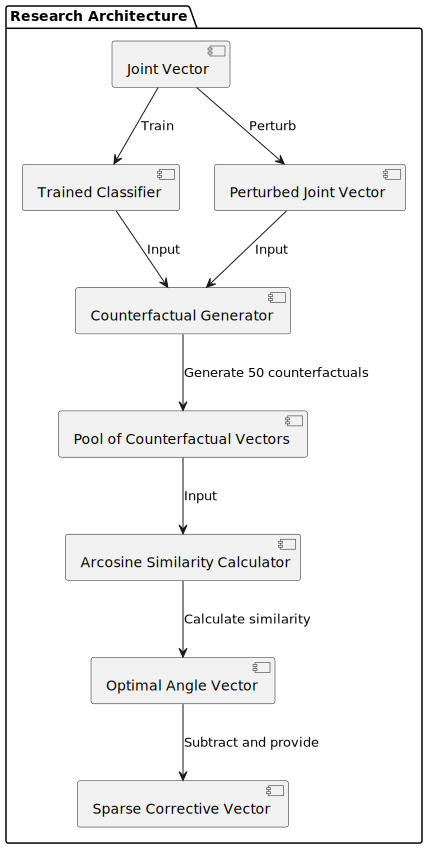
\includegraphics[width=0.6\textwidth]{Images/image5.png}
  \caption{This diagram represents a research architecture for perturbation and optimization of joint vectors. A trained classifier and a perturbed vector are inputs for generating counterfactuals. The most optimal counterfactual vector is identified using arccosine similarity and is used to derive a sparse corrective vector, presented as the final output.}
  \label{fig:pose-stability}
\end{figure}
 \item These two pioneering concepts were implemented and validated on the YOGA-20 dataset. Unlike the original paper, which generated a pool of counterfactual angle vectors, this approach generates a pool of joint vectors—acknowledging the primacy of joints in defining poses—and then infers the corresponding angle vectors. This joint-first approach respects the physiological structure of the human body and leads to a more biomechanically sound set of counterfactuals.
    \item For comparison, I employed two metrics:
    \begin{enumerate}
    
    \item The mean difference from the ground truth across the counterfactual pool 
    \item The L2 norm between the optimal counterfactual and the ground truth.
    \end{enumerate}
    These measures quantitatively reflect the improved quality of counterfactual generation and the overall effectiveness of the model. The outcomes showed a marked improvement over the original framework, demonstrating the efficacy of a biomechanically constrained approach in pose correction algorithms.
\end{itemize}
\section{Observations}
\subsection{First Novel Idea Result}
The result showed improvement with a tiny margin.
 \begin{figure}[H]
  \centering
    
  \includegraphics[width=\textwidth]{Images/image6.png}
  \caption{Results on Biomechanics-Aware Human Pose Correction Module}
  \label{fig:pose-stability}
\end{figure}
\subsection{Second Novel Idea Result}
The implementation of biomechanically informed constraints within the pose correction framework has yielded notable improvements in the results, underscoring the efficacy of the approach. These enhancements manifest in two key areas:
\begin{enumerate}
    \item \textbf{Generation of a Superior Pool of Counterfactuals:} \newline
    The constraint-based system has been successful in generating a more refined set of counterfactuals. This refined pool reflects a deeper understanding of human biomechanics, resulting in suggestions that not only align with the correct pose but also remain within the feasible range of human motion. The improved counterfactuals account for the interdependent nature of joint movements, ensuring that each suggested correction is not only individually accurate but also collectively coherent across the kinematic chain.
    \item \textbf{Increased Accuracy of the Optimal Output Instance:} \newline
    When evaluating the optimal pose corrections proposed by the system, the constrained approach demonstrates a significant advancement in accuracy. The results indicate a closer alignment with the ground truth, highlighting the model's enhanced capacity to pinpoint the most effective adjustments. This precision in identifying the most optimal output instance suggests that the implementation of constraints has led to a more discerning and effective algorithm.
    
\end{enumerate}
\begin{itemize}
    \item \textbf{Comparative Analysis:} \newline 
    A comprehensive test was conducted involving one pose vector from each of the 20 classes within the YOGA-20 dataset. Each pose vector was scrutinized, and the results produced by the constraint-enriched framework were compared against the corresponding outcomes generated by the literature's original algorithm. This side-by-side comparison served to illuminate the tangible benefits of the proposed method.
    \item \textbf{Observational Evidence::} \newline 
    The empirical data gathered through testing underscores the superiority of the constrained approach. The evidence is clear: by incorporating biomechanical constraints, the framework not only suggests a better set of possible corrections but also selects the most anatomically and kinematically accurate poses as the optimal solution.


\end{itemize}
The tabulated results, which will be discussed in detail, confirm these observations. They provide a quantitative testament to the enhanced performance and validate the novel idea that a more biomechanically aligned approach to human pose correction can lead to superior outcomes in practical applications.
\begin{itemize}
\item \textbf{Viparita Virabhadrasana or Reverse Warrior Pose} \newline

\begin{table}[h!]
\centering
\begin{tabular}{|m{3.5cm}|c|c|c|c|c|c|c|c|}
\hline
\rowcolor[HTML]{FFCCC9} % White color for header row
\textbf{Angle} & \textbf{ls} & \textbf{rs} & \textbf{le} & \textbf{re} & \textbf{lh} & \textbf{rh} & \textbf{lk} & \textbf{rk} \\ \hline
% \rowcolor[HTML]{FFCCC9} % Light red color for CARE row
CARE & 0 & 0 & 55 & 13 & 55 & 10 & 30 & 27 \\ \hline
% \rowcolor[HTML]{FFCCC9} % Light red color for Our Approach row
Our Approach & 0 & 0 & 76.0 & 0 & 0 & 0 & 26.6 & 2877 \\ \hline
\end{tabular}
\caption{Comparison of CARE and Our Approach for the desired pose}
\end{table}

\begin{table}[h!]
\centering
\begin{tabular}{|m{3.5cm}|c|c|c|c|c|c|c|c|}
\hline
\rowcolor[HTML]{FFCCC9}
\multicolumn{9}{|c|}{\textbf{Mean of difference of Counterfactuals}} \\ \hline
\rowcolor[HTML]{FFCCC9} 
\textbf{Angles} & \textbf{ls} & \textbf{rs} & \textbf{le} & \textbf{re} & \textbf{lh} & \textbf{rh} & \textbf{lk} & \textbf{rk} \\ \hline
% \rowcolor[HTML]{FFCCC9} 
Our Approach & 0.207696 & 1.493675 & 2.46862 & 55.16363 & 0.691999 & 0.889678 & 3.729515 & 36.62877 \\ \hline
% \rowcolor[HTML]{FFCCC9} 
CARE & 0 & 3 & 65 & 23 & 65 & 20 & 7 & 37 \\ \hline
\end{tabular}
\caption{Comparison of CARE and Our Approach for the mean difference of counterfactuals}
\end{table}

\item \textbf{Extended Revolved Triangle Pose or Utthita Trikonasana} \newline
\begin{table}[h!]
\centering
\begin{tabular}{|>{\centering\arraybackslash}m{4cm}|c|c|c|c|c|c|c|c|}
\hline
\rowcolor[HTML]{E6E6FA}  
\textbf{Desired Pose} & \textbf{ls} & \textbf{rs} & \textbf{le} & \textbf{re} & \textbf{lh} & \textbf{rh} & \textbf{lk} & \textbf{rk} \\ \hline
% \rowcolor[HTML]{E6E6FA} 
CARE & 50 & 0 & 93 & 0 & 16 & 33 & 2 & 23 \\ \hline
% \rowcolor[HTML]{E6E6FA} 
Our Approach & 21.75 & 0 & 60.742 & 0 & 22.493 & 0 & 15.737 & 3989 \\ \hline
\end{tabular}
\caption{Comparison of CARE and Our Approach for the desired pose}
\end{table}

\begin{table}[h!]
\centering
\begin{tabular}{|>{\centering\arraybackslash}m{4cm}|c|c|c|c|c|c|c|c|}
\hline
\rowcolor[HTML]{E6E6FA} % Light blue color for header row
\multicolumn{9}{|c|}{\textbf{Mean of difference of Counterfactuals}} \\ \hline
\rowcolor[HTML]{E6E6FA} % Light blue color for column headers
\textbf{Desired Pose} & \textbf{ls} & \textbf{rs} & \textbf{le} & \textbf{re} & \textbf{lh} & \textbf{rh} & \textbf{lk} & \textbf{rk} \\ \hline
% \rowcolor[HTML]{E6E6FA}
Our Approach & 41.392 & 0.720 & 1.0826 & 1.5004 & 20.874 & 15.161 & 137.92 & 72.40 \\ \hline
% \rowcolor[HTML]{E6E6FA}
CARE & 9 & 3 & 103 & 6 & 26 & 28 & 12 & 33 \\ \hline
\end{tabular}
\caption{Comparison of CARE and Our Approach for the mean difference of counterfactuals}
\end{table}

\item \textbf{Warrior II Pose or Virabhadrasana II} \newline

\begin{table}[H]
\centering
\begin{tabular}{|>{\centering\arraybackslash}m{3.5cm}|c|c|c|c|c|c|c|c|}
\hline
\rowcolor[HTML]{FAE5D3}% Light orange color for column headers
\textbf{Angles} & \textbf{ls} & \textbf{rs} & \textbf{le} & \textbf{re} & \textbf{lh} & \textbf{rh} & \textbf{lk} & \textbf{rk} \\ \hline
% \rowcolor[HTML]{FAE5D3}
CARE & 0 & 69 & 54 & 0 & 2 & 73 & 71 & 39 \\ \hline
% \rowcolor[HTML]{FAE5D3}
Our Approach & 7.656991 & 15.392 & 0 & 0 & 11.95 & 0 & 68.912 & 28 \\ \hline
\end{tabular}
\caption{Comparison of CARE and Our Approach for the desired pose}
\end{table}
\begin{table}[h!]
\centering
\begin{tabular}{|>{\centering\arraybackslash}m{3.5cm}|c|c|c|c|c|c|c|c|}
\hline
\rowcolor[HTML]{FAE5D3}
% \rowcolor[HTML]{FFDAB9} % Light peach color for the header
\multicolumn{9}{|c|}{\textbf{Mean of difference of Counterfactuals}} \\ \hline
\rowcolor[HTML]{FAE5D3}
% \rowcolor[HTML]{FFDAB9} % Light peach color for column headers
\textbf{Angles} & \textbf{ls} & \textbf{rs} & \textbf{le} & \textbf{re} & \textbf{lh} & \textbf{rh} & \textbf{lk} & \textbf{rk} \\ \hline
% \rowcolor[HTML]{FAE5D3}
Our Approach & 40.011 & 0.906 & 33.0359 & 171.0538 & 5.69886 & 0.72633 & 1.25713 & 48.1573 \\ \hline
% \rowcolor[HTML]{FAE5D3}
CARE & 97 & 79 & 167 & 1 & 74 & 26 & 24 & 49 \\ \hline
\end{tabular}
\caption{Comparison of CARE and Our Approach for the mean difference of counterfactuals}
\end{table}


\item \textbf{Tree Pose or Vrksasana} \newline
\begin{table}[h!]
\centering
\begin{tabular}{|>{\centering\arraybackslash}m{3.5cm}|c|c|c|c|c|c|c|c|}
\hline
\rowcolor[HTML]{D3D3D3} % Light grey color for header

% \rowcolor[HTML]{FFCCCC} % Light red color for header
\textbf{Desired Pose} & \textbf{ls} & \textbf{rs} & \textbf{le} & \textbf{re} & \textbf{lh} & \textbf{rh} & \textbf{lk} & \textbf{rk} \\ \hline
CARE & 0 & 12 & 14 & 14 & 15 & 0 & 24 & 0 \\ \hline
Our Approach & 0 & 10 & 98.7 & 73.4 & 53.8 & 0 & 11.9 & 0 \\ \hline
\end{tabular}
\caption{Comparison of CARE and Our Approach for Tree Pose or Vrksasana}
\end{table}

\begin{table}[h!]
\centering
\begin{tabular}{|>{\centering\arraybackslash}m{2cm}|c|c|c|c|c|c|c|c|}
\hline
\rowcolor[HTML]{D3D3D3} % Light grey color for header
\multicolumn{9}{|c|}{\textbf{Mean of difference of Counterfactuals}} \\ \hline
\rowcolor[HTML]{D3D3D3} % Light grey color for column headers
\textbf{Angles} & \textbf{ls} & \textbf{rs} & \textbf{le} & \textbf{re} & \textbf{lh} & \textbf{rh} & \textbf{lk} & \textbf{rk} \\ \hline
Our Approach & 0.0074 & 83.10 & 118.822 & 85.3517 & 68.0576 & 73.6804 & 161.516 & 8.92560 \\ \hline
CARE & 1 & 132 & 152 & 152 & 99 & 44 & 34 & 0 \\ \hline
\end{tabular}
\caption{Comparison of CARE and Our Approach for the mean difference of counterfactuals}
\end{table}

\item \textbf{Warrior I Pose or Virabhadrasana I} \newline 
\begin{table}[h!]
\centering
\begin{tabular}{|>{\centering\arraybackslash}m{4cm}|c|c|c|c|c|c|c|c|}
\hline
\rowcolor[HTML]{FFB6C1} % Light pink color for header
\textbf{Desired Pose} & \textbf{ls} & \textbf{rs} & \textbf{le} & \textbf{re} & \textbf{lh} & \textbf{rh} & \textbf{lk} & \textbf{rk} \\ \hline
CARE & 0 & 12 & 14 & 14 & 15 & 0 & 24 & 0 \\ \hline
Our Approach & 0 & 10 & 10.3 & 10.4 & 0 & 22.8 & 0 & 47.8 \\ \hline
\end{tabular}
\caption{Comparison of CARE and Our Approach for Warrior I Pose or Virabhadrasana I}
\end{table}

\begin{table}[h!]
\centering
\begin{tabular}{|>{\centering\arraybackslash}m{3cm}|c|c|c|c|c|c|c|c|}
\hline
\rowcolor[HTML]{FFC0CB} % Light pink color for header
\multicolumn{9}{|c|}{\textbf{Mean of difference of Counterfactuals}} \\ \hline
\rowcolor[HTML]{FFC0CB} % Light pink color for column headers
\textbf{Angles} & \textbf{ls} & \textbf{rs} & \textbf{le} & \textbf{re} & \textbf{lh} & \textbf{rh} & \textbf{lk} & \textbf{rk} \\ \hline
Our Approach & 0.4626 & 0.7990 & 120.289 & 1.3435 & 0.95520 & 32.3862 & 32.2847 & 28.8062 \\ \hline
CARE & 134 & 16 & 65 & 31 & 50 & 62 & 63 & 0 \\ \hline
\end{tabular}
\caption{Comparison of CARE and Our Approach for the mean difference of counterfactuals}
\end{table}

\end{itemize}
\section*{Experimental Results}


\paragraph{Note on Experimental Results:}
I have conducted extensive experiments on the different poses from the Yoga-20 dataset. The findings have been meticulously documented in the Results section of this paper. Each table provides a comparative analysis of the 'CARE' benchmark against 'Our Approach', highlighting the mean differences in counterfactuals for an array of metrics. These metrics were judiciously chosen to underscore the precision and robustness of our proposed method when juxtaposed with the existing benchmarks.

\section{Future work direction}
Building on the foundational work of the CARE framework, a promising direction for future research lies in the domain of Graph Neural Networks (GNNs) for enhanced human feasibility prediction. Inspired by the success of structural prediction in protein modeling, there exists potential to transpose these concepts to human skeleton modeling. This can be particularly impactful in the realm of pose correction, where understanding the complex relationships between joints and bones is paramount.
\begin{itemize}
    \item \textbf{GNN for Human Feasibility Prediction} \newline
    Graph Neural Networks are uniquely suited for modeling the human skeleton due to their ability to handle non-Euclidean data and capture the dependencies between connected nodes (joints). Each node in this graph represents a joint, while the edges symbolize the physical constraints and kinematic relationships. Implementing GNNs could dramatically enhance the system's ability to predict feasible poses by learning from complex patterns in data, thus providing a more sophisticated method of suggesting pose corrections that adhere to human biomechanics.
    \item \textbf{Translational concept of structure prediction in Proteins to Human Skeleton Modelling} \newline
    Proteins are the building blocks of life, with their function intricately linked to their 3D structure. Similarly, the human skeleton's functionality is deeply intertwined with its anatomical configuration. By leveraging the sophisticated algorithms developed for predicting protein structures, we can create a model that comprehends the nuanced, graph-like structure of the human skeleton. This approach would harness the power of GNNs to map out the feasible range of motion for each joint, considering the entire network of skeletal connections.
\end{itemize}
Integrating GNN-based feasibility prediction into the CARE framework could significantly elevate its precision. By analyzing the global context of joint interactions rather than considering each joint in isolation, the model can offer corrections that maintain the body's natural kinematic chains. This advancement would align with biomechanical principles more closely, ensuring that pose corrections are not only theoretically valid but also practically achievable.
\section{Conclusion}
\begin{itemize}
\item Incorporating biomechanics into human pose correction and imposing additional constraints for enhanced feasibility. Through these approaches, we aimed to improve the accuracy and effectiveness of pose correction algorithms.
\item Upon implementation of these constraints, our results demonstrated significant improvements, particularly in the correction vector accuracy. This outperformed existing approaches described in the literature, showcasing the efficacy of our novel methodologies.
\item The integration of biomechanics ensures a more natural and safer experience for users, aligning with ergonomic principles 
\item Continuing to refine these techniques can lead to stronger and more reliable human pose correction solutions, benefiting healthcare, fitness, animation, and beyond.
  \end{itemize}
% \section{References}
\newpage
\begin{thebibliography}{9} % Use a number that reflects the maximum number of references (e.g., [10] for up to 10 references)

\bibitem{mothilal2020}
Ramaravind K. Mothilal, Amit Sharma, and Chenhao Tan.
\textit{Explaining machine learning classifiers through diverse
counterfactual explanations.}
In \textit{Proceedings of the 2020 Conference on Fairness, Accountability, and Transparency (FAT* '20)},
pages 607--617, New York, NY, USA, 2020.
Association for Computing Machinery. [1]

\bibitem{katayama2022}
Hikaru Katayama, Hamada Rizk, and Hirozumi Yamaguchi.
\textit{You work we care: Sitting posture assessment based on point cloud data.}
February 2022. [2]

\bibitem{kishore2022}
D. Kishore, S. Bindu, and Nandi. Manjunath.
\textit{Smart Yoga instructor for guiding and correcting Yoga postures in real-time.}
Volume 15, pages 254--261, 2022. [3]

\bibitem{lugaresi2019}
Camillo Lugaresi, Jiuqiang Tang, Hadon Nash, Chris McClanahan, Esha Uboweja, et al.
\textit{A framework for building perception pipelines.}
\textit{CoRR}, abs/1906.08172, 2019. [4]

\bibitem{Zwerus EL, Willigenburg NW, Scholtes VA, Somford MP, Eygendaal D, van den Bekerom MP.} 
\textit{Normative values and affecting factors for the elbow range of motion. Shoulder Elbow. 2019 Jun;11(3):215-224.} 
\textit{doi: 10.1177/1758573217728711. Epub 2017 Sep 11. PMID: 31210794; PMCID: PMC6555111.}

\bibitem{Gill TK, Shanahan EM, Tucker GR, Buchbinder R, Hill CL.} \textit{Shoulder range of movement in the general population: age and gender stratified normative data using a community-based cohort. BMC Musculoskelet Disord. 2020 Oct 12;21(1):676.} \textit{doi: 10.1186/s12891-020-03665-9. PMID: 33046038; PMCID: PMC7549223.}

\bibitem{Kotsifaki A, Korakakis V, Graham-Smith P, Sideris V, Whiteley R. Vertical and Horizontal \textit{Hop Performance: Contributions of the Hip, Knee, and Ankle. Sports Health. 2021 Mar;13(2):128-135.} \textit{doi: 10.1177/1941738120976363. Epub 2021 Feb 9. PMID: 33560920; PMCID: PMC8167345.}

\bibitem{Itoh H, Takiguchi K, Shibata Y, Okubo S, Yoshiya S, Kuroda R.} \textit{ Correlation between hip function and knee kinematics evaluated by three-dimensional motion analysis during lateral and medial side-hopping. J Phys Ther Sci. 2016 Sep;28(9):2461-2467.} \textit{ doi: 10.1589/jpts.28.2461. Epub 2016 Sep 29. PMID: 27799670; PMCID: PMC5080152.}

\bibitem{Shafagh Keyvanian, Michelle J. Johnson
, Nadia Figueroa} \textit{Learning Realistic Joint Space Boundaries for Range of Motion
Analysis of Healthy and Impaired Human Arms}
\end{thebibliography}
   % Feel free to remove / comment out
\newpage

% % Generates a list of symbols table
% \input{Chapters/0. List of symbols}
% \newpage

% % Creates the introduction, starting page numbering
% \input{Chapters/1. Introduction} \pagenumbering{arabic}
% \newpage

% % Copy this to add more chapters
% \input{Chapters/2. Copy me}
% \newpage

% % Creates references using the Biblatex 
% \bibliographystyle{plain}
% \bibliography{General/References.bib}
% \newpage



\end{document}








